\section{Versuch 5 - Ermittlung des Reibwertes $C_{\psi}$}
Im nächsten Versuchsaufbau wird die Würfelseite fixiert ($\dot{\varphi} = 0$). Hierbei beschleunigt der Motor die Schwungmasse mit einem konstanten Drehmoment $T_M=10mNm$. $T_M$ ist so zu wählen, dass sich die Radgeschwindigkeit $\dot{\psi}$ in einem Bereich bewegt, welcher dem Arbeitsbereich des geschlossenen Regelkreises entspricht. 

\begin{figure}[h!]
\centering
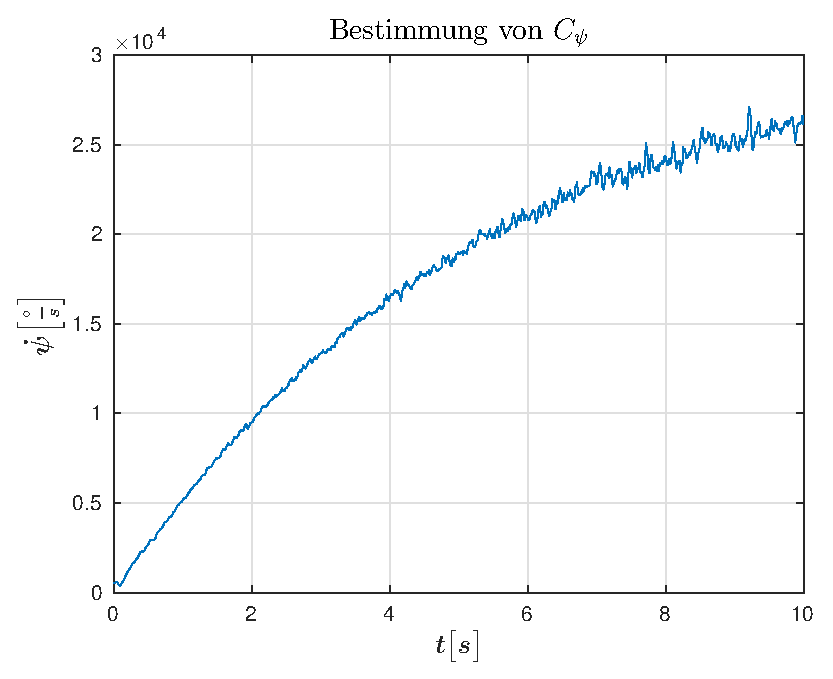
\includegraphics[width=0.6\linewidth]{img/C_psi.eps}
\caption{Versuch 5: Verlauf der Radgeschwindigkeit, Quelle: eigene Darstellung}
\end{figure}


Da die Bewegung auf einen Freiheitsgrad beschränkt wurde vereinfacht sich das Modell des Systems auf die folgende Bewegungsgleichung.

\begin{equation}
\label{ermittlung_c_psi_equation}
\theta^B_R \cdot \ddot{\psi} = T_M - C_\psi \cdot \dot{\psi}
\end{equation}

Im Versuchsverlauf werden bei $n$ Stützstellen die Werte von $\psi$, $\dot{\psi}$ und $\ddot{\psi}$ gemessen. Daraus ergeben sich die folgenden Vektoren.

\begin{equation}
\label{ermittlung_c_psi_vektoren_equation}
\boldsymbol{\psi} = \begin{pmatrix} \psi_1 \\ \psi_2 \\ \vdots \\ \psi_n \end{pmatrix} \hspace{35pt}
\boldsymbol{\dot{\psi}} = \begin{pmatrix}
\dot{\psi_1} \\ \dot{\psi_2} \\ \vdots \\ \dot{\psi_n}
\end{pmatrix} \hspace{35pt}
\boldsymbol{\ddot{\psi}} = \begin{pmatrix}
\ddot{\psi_1} \\ \ddot{\psi_2} \\ \vdots \\ \ddot{\psi_n}
\end{pmatrix}
\end{equation}

Durch Einsetzen von \ref{ermittlung_c_psi_vektoren_equation} in \ref{ermittlung_c_psi_equation} kann über die Methode der kleinsten Fehlerquadrate wiederum der Reibwert $C_\psi$ bestimmt werden.

\begin{equation}
C_{\psi}= 4.8301 \cdot 10^{-6} \cdot kg \cdot m^2 \cdot s^{-1}
\end{equation}